\documentclass[12pt]{article}

\usepackage{amsmath, amssymb, amsthm}
\usepackage{graphicx}	% use to include graphics
\usepackage{verbatim}
\usepackage{multicol}

\makeatletter
\renewcommand\section{\@startsection{section}{1}{\z@}%
								 {-3.5ex \@plus -1ex \@minus -.2ex}%
								 {2.3ex \@plus.2ex}%
								 {\normalfont\large\bfseries}}
\makeatother

\title{CSE 490h Assignment 3}
\author{
Colin Scott and Bill Cauchois \\
}

%%%%%%%%%%%%%%%%%%%%%%%%%%%%%%%%%%%%%%%%%%%%%%%%%%%%%%%%%%%%%%%%%%%%%%%%%%%%%%%%%%%%%
\begin{document}
\maketitle

In this assignment we added transactions to our distributed, cache coherent system. Transactions ensure atomicity, consistency, isolation, and durability (ACID). We describe how these properties are enforced on the clients, and on the centralized manager (this topology is carried over from the last assignment).

\section{Overview}

We describe our system in two parts. First, we describe the operation of the server, whose responsibility it is to maintain a canonical copy of each file in the cache as well as certain per-file state. The server also maintains an undo log to maintain consistency. Then, we describe the operation of the client, which is responsible for receiving instructions from the application layer, bundling them into transactions (while performing certain operations on a local copy of the distributed cache), and submitting them to the server which may accept or reject them.

\subsection{Properties of Our System}

\begin{itemize}
\item We guarantee linearizability for client and server operations. For example, if the client executes put A, get B, the get B will not be executed until the put A has fully completed.
\item We implement a version of write-through caching. You can think of it as a weak form of optimistic concurrency control.
\item The server keeps authoritative copies of all files.
\item Each authoritative copy has an associated version number
\item When a client sends a transaction to the server, the server first checks that each of the files involved in the transaction is up-to-date.
\item If one of the files is out-of-date, a concurrency error has occurred. In this case the server will notify the client that the transaction did not complete successfully, and the client will flushes its cache
\item If all files are up-to-date, the server begins executing the transaction
\item We use an undo log to rollback transactions on the server
\item If an exception occurs while the server executes the transaction, the server rolls back, and notifies the client that the transaction did not go through.
\item Finally, if the transaction goes through successfully, the authoritative copies on the server are updated.
\item The client keeps files in its cache between transactions. We use callbacks to invalidate out-of-date cache entries. If a client receives an invalidatoin request while processing a transaction, it immediately aborts. This is an optimization -- we know that the transaction will fail when it get to the server since the version number is out-of-date.
\end{itemize}

\section{Serverside}

\subsection{State}

The server maintains authoritative copies of each file. In addition to the contents of each file, the server also stores a \emph{version} and a \emph{copyset} for each file (this latter concept is carried over from the last assignment). Versioning is necessary because clients' local cache may contain out-of-date copies of the files, depending on how messages are delayed. A copyset is necessary because clients' local copies of a file must be invalidated whenever another client writes to that file.

\subsection{Transactions}

Transactions are always submitted by clients in a bundle consisting of a list of \textsc{Update} messages. An \textsc{Update} message has a type: one of \{\textsc{Write}, \textsc{Read}, \textsc{Create}, \textsc{Delete}\}, as well as a filename, version, and a contents buffer. Basically, an \textsc{Update} encapsulates an operation by the client on a file. A transaction, then, is just a list of \textsc{Updates} that must be executed atomically.

The server's job is to receive a transaction in a \textsc{CommitAttempt} message, determine whether that transaction is valid, and if so, execute it. We then notify the client whether their transaction succeeded.

In order to determine whether a transaction is valid, we check the version in each \textsc{Update} message (which represents the version that the client has) against the version of our canonical copy on the server. If there's a mismatch, then the client is operating with an out-of-date version of the file and its transaction fails. A transaction may also fail if there is an IO exception.

\subsection{Executing a Transaction}

Executing the transaction is a subtle affair because we must ensure consistency. That is, if the server fails while executing its transaction it must be able to recover to a consistent state. We achieve consistency using an undo log (described in the next section), but first we describe how transactions are executed.

A transaction is executed on the server by iterating through the list of \textsc{Update}s and executing each in turn. Executing an \textsc{Update} consists of three steps:

\begin{enumerate}
\item Logging the action we are about to perform.
\item Updating our in-memory state (namely, the file table; for example, for a \textsc{Write}, we will increment the version number of the file to reflect that a change to that file has occurred).
\item Updating our cache on the filesystem.
\end{enumerate}

Note that the transaction is not officially comitted until we write the commit to the undo log. When all of the updates have been executed successfully, we do so. Finally, we send invalidate requests out to the copysets of all files that have been modified by the transaction. Then, we can send a successful response to the client (which contains the new version numbers for each modified file).

If at any point during the transaction the server crashes, we need to ensure that the state of all files is consistent. This is accomplished by the undo log.

\subsection{Undo Logging}

With an undo log, we log the necessary data to restore a file to its original state in the event that a transaction fails. This functionality is encapsulated in a separate class that handles serializing and deserializing log messages, as well as recovering from a failure.

To recover from a failure, we read the log starting from the bottom and find the latest uncommitted transaction. Then, we restore the original state of every file for that transaction. This effectively rolls back the transaction and ensures a consistent state.

\section{Clientside}

Clients maintain their own caches. Local caches provide two major benefits:
\begin{enumerate}
\item They help minimize communication with the server. For example, the client may reuse files in its cache in between transactions without having to go to the server to get a new copy.
\item If a transaction is computationally expensive, the client can perform the computations independently of the server, only sending a final `summary' of the modifications to be processed centrally.
\end{enumerate}

\subsection{Transaction Summarization}

To `summarize' the transaction, we devised the following state machine:

\begin{center}
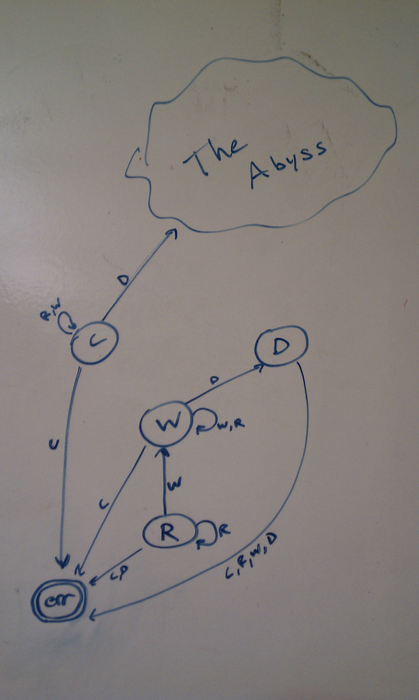
\includegraphics[width=300px]{a3_states.png}
\end{center}

As the transaction proceeds, each file makes state transitions as above. The `summary' we send to the server then is just the final state of each file, along with the initial version and the most recent contents. 

Note that `The Abyss' denotes a NULL operation -- the client does not need to notify the server of a create followed by a delete.

The client optimistically makes changes to its cache immediately. If an error occurs, all files relevant to the current transaction are flushed from the cache.

If the client performs a get() or a put(), and the file is not currently in the cache, the client asks for the latest authoratative copy from the server. Creates and deletes do not require communication with the server. We initially viewed this as an optimization, but in retrospect we regret this particular design decision.

\subsection{Design Notes}

\begin{itemize}
\item If the user enters a command which is not surrounded by `txstart' and `txcommit', we execute their command as a single operation transaction.
\item We decided to disallow a delete followed by a create on the client, as this radically simplifies our implementation. We believe this decision is justified because a delete followed by a create is exactly equivalent to a put of the empty string.
\item There are cases where the server may crash before it has time to respond to a client request. To deal with this situation, we implemented probing in our RIO layer, such that each OutConnection sends out a heartbeat message every 6 rounds. If we ever detect that the server has a different instance identifier, the RIO layer will notify the client that the server has crashed. Then, the client can abort any pending transactions.
\end{itemize}

\section{Example}

We present a short example to illustrate the operation of our system. Suppose that the server has two authoritative files: foo.txt, version 3; and bar.txt, version 1. Consider two clients executing concurrent transactions on both files. Suppose the following sequence of events occurs. Client 1 and 2 begin their transactions. Client 1 executes get foo.txt, and finds that it has the file in its cache already. Client 2 executes put bar.txt but does not have the file in its cache, and subsequently requests the authoritative copy from the server. Client 1 executes put bar.txt. Upon receipt of the authoritative copy, client 2 executes put foo.txt. Finally, client 1 sends the commit summary to the server. The server sees that all the versions are up-to-date, and updates its global state accordingly. In doing so, it sees that client 2 was in the copyset of foo.txt, and sends an invalidate request to client 2. Client 2, upon receiving the invalidation request, sees that it has an outdated version and immediately aborts.

\section{Wishlist}

There are certain features we wish we could have implemented, if we had had the time:

\begin{itemize}
\item We do not make a distinction between concurrency errors and operation exceptions; we treat transcations as `all-or-nothing'. Vincent pointed out in lecture that a transaction might still go through if one operation throws an exception, but we were not conceptualizing transactions in this way when we implemented our server. In retrospect, the distinction seems useful.
\item If an error occurs, e.g., \textsc{FILE\_ALREADY\_EXISTS}, the server passes back a \emph{single} error code for the entire transaction. As such, the user has no way of knowing which operation the \textsc{FILE\_ALREADY\_EXISTS} error corresponds to. This problem would be solved if we had complied with Vincent's distinction between concurrency errors and operation exceptions.
\item We may abort some transactions when it's not strictly necessary to do so. For example, it might be possible in some cases to assign a virtual time to a particular transaction ''in the past``, so that two concurrent transactions do not conflict. For this implementation we decided that the benefit of this optimization outweighed the complexity cost.
\end{itemize}

\end{document}

